\begin{figure}[h!]
	\centering
	\begin{minipage}[b]{1\textwidth}
    		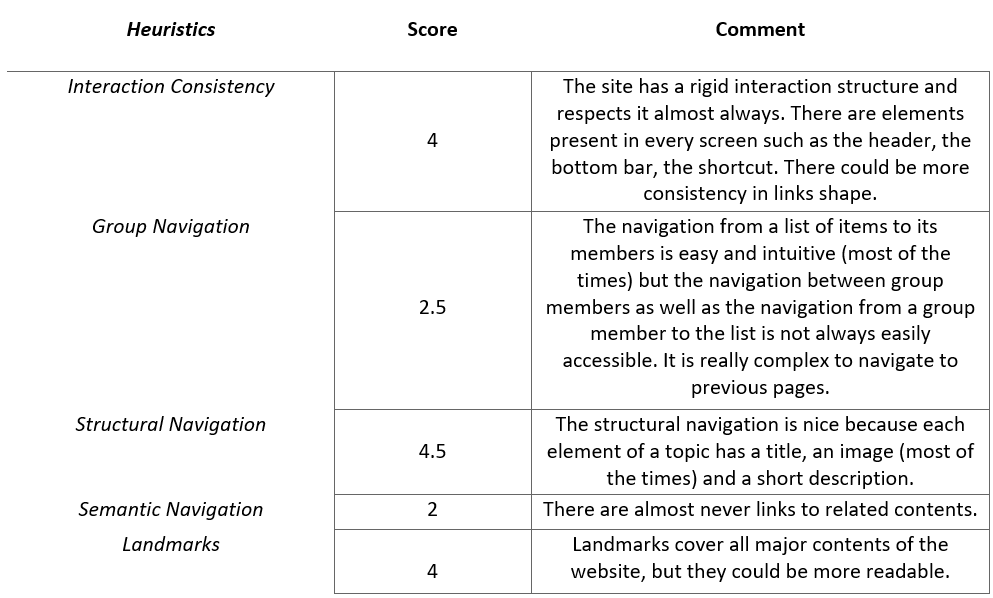
\includegraphics[width=\textwidth]{./assets/navigation-final.PNG}
	\end{minipage}
\end{figure}
\FloatBarrier
\subsubsection{Interaction Consistency}
This website has a pretty consistent choice of interaction. Every page shares the following elements:
\begin{itemize}
	\item \textbf{Header:} gives the possibility to change language, season and to access to the newletter page (fig. 1) ;
	\item \textbf{Topbar:} allows a user to navigate between almost every website page and content , it is the main navigation 		instrument (fig. 2); 
	\item \textbf{Leftbar:} let a user to get important information such as weather, skilift 	situation, online skipass booking (fig. 		3);
	\item \textbf{Footer:} provides links to partners' websites, to its social network profiles and general informations such as 			contacts and privacy policies (fig. 4).
\end{itemize}  

\begin{figure}[h!]
	\centering
	\begin{minipage}[b]{0.7\textwidth}
    		
\includegraphics[width=\textwidth]{./assets/Interaction-header.png}
		\caption{Header}
	\end{minipage}
	\hfill
	\centering
	\begin{minipage}[b]{0.7\textwidth}
    		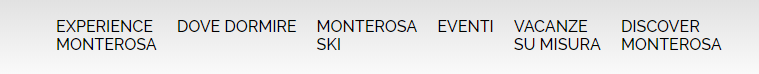
\includegraphics[width=\textwidth]{./assets/Interaction-topbar.png}
		\caption{Topbar}
	\end{minipage}
\end{figure}
\FloatBarrier

\begin{figure}[h!]
	\centering
	\begin{minipage}[b]{0.28\textwidth}
    		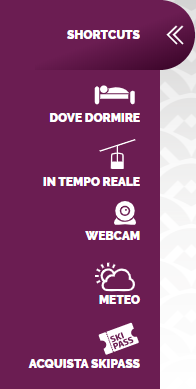
\includegraphics[width=\textwidth]{./assets/Interaction-leftbar.png}
		\caption{Leftbar}
	\end{minipage}
	\hfill
	\begin{minipage}[b]{0.65\textwidth}
    		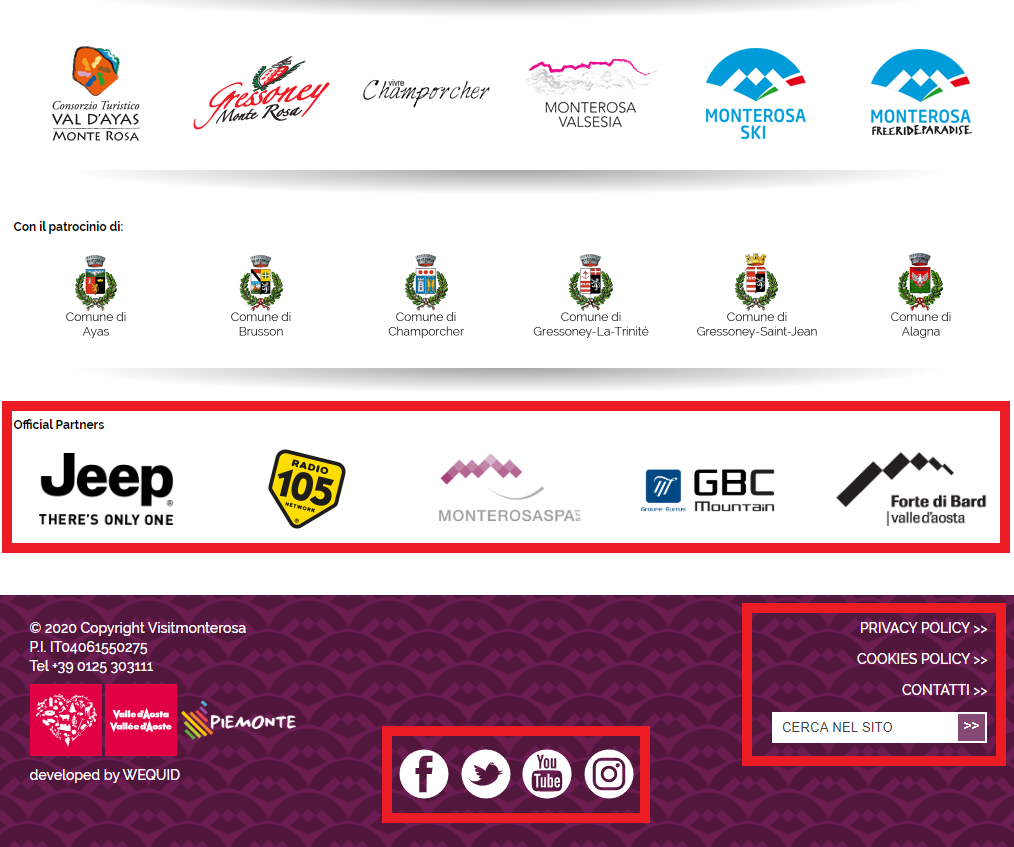
\includegraphics[width=\textwidth]{./assets/Interaction-bottom-bar.png}
		\caption{Footer}
	\end{minipage}
\end{figure}
\FloatBarrier

\subsubsection{Group Navigation}
\begin{wrapfigure}{r}{0.2\textwidth}
    	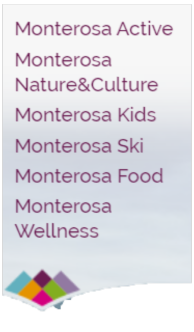
\includegraphics[width=0.9\linewidth]{./assets/dropdown-menu.png}
	\caption{Dropdown Menù}
\end{wrapfigure} Thanks to the Header (fig 1.) and the Leftbar (fig. 3) a quick access is granted to almost all possible contents. Group navigation is also supported by header's dropdown menù (fig. 5), which contain the links to all main components of each group and helps the user to navigate between them. 

\subsubsection{Structural Navigation}


\subsubsection{Semantic Navigation}
Semantic navigation is provided with links to the related pages that can be found for example in dropdown menu (fig. 5). Even though almost all contents can be accessed through the header, it is not possible to easily navigate between related contents in an easy way bacause , except for some pages, similar contents aren't connect via a visible link. User can get confused also because there are also some links with an equivalent text label that bring to different pages with different contents, 

\subsubsection{Landmarks}
Landmarks can be found into the four elements described in "Interaction Concistency" paragraph. These elements are static becauee they do not change between different pages, but they could be more effective by adopting some customization.